% TEMPLATE.TEX
%
% Time-stamp: <2013-03-26 11:09 olenz>
%
% This is an extensively documented LaTeX file that shows how to
% produce a good-looking document with current LaTeX (11/2012).
%
% IMPORTANT!
%
%   Some obsolete commands and packages
% ----------|-------------------------------
% obsolete  |     Replacement in LATEX 2ε
% ----------|-------------------------------
%           | local            global/switch
% ----------|-------------------------------
% {\bf ...} | \textbf{...}     \bfseries
%     -     | \emph{...}       \em
% {\it ...} | \textit{...}     \itshape
%     -     | \textmd{...}     \mdseries
% {\rm ...} | \textrm{...}     \rmfamily
% {\sc ...} | \textsc{...}     \scshape
% {\sf ...} | \textsf{...}     \sffamily
% {\sl ...} | \textsl{...}     \slshape
% {\tt ...} | \texttt{...}     \ttfamily
%     -     | \textup{...}     \upshape
%
% DON'T USE \\ TO MAKE LINEBREAKS, INSTEAD JUST LEAVE A BLANK LINE!
%
\RequirePackage[l2tabu,orthodox]{nag} % turn on warnings because of bad style
\documentclass[a4paper,10pt,bibtotoc]{scrartcl}
%
\usepackage[bottom=3.5cm, top=1cm]{geometry}
%%%%%%%%%%%%%%%%%%%%%%%%%%%%%%%%%%%%
% KOMA CLASSES
%%%%%%%%%%%%%%%%%%%%%%%%%%%%%%%%%%%%
%
% The class "scrartcl" is one of the so-called KOMA-classes, a set of
% very well done LaTeX-classes that produce a very European layout
% (e.g. titles with a sans-serif font).
%
% The KOMA classes have extensive documentation that you can access
% via the commands:
%   texdoc scrguide # in German
%   texdoc scrguien # in English
%
%
% The available classes are:
%
% scrartcl - for "articles", typically for up to ~20 pages, the
%            highest level sectioning command is \section
%
% scrreprt - for "reports", typically for up to ~200 pages, the
%            highest level sectioning command is \chapter
%
% scrbook  - for "books", for more than 200 pages, the highest level
%            sectioning command is \part.
%
% USEFUL OPTIONS
%
% a4paper  - Use a4 paper instead of the default american letter
%            format.
%
% 11pt, 12pt, 10pt
%          - Use a font with the given size.
%
% bibtotoc - Add the bibliography to the table of contents
%
% The KOMA-script classes have plenty of options to modify

% This allows to type UTF-8 characters like ä,ö,ü,ß
\usepackage[utf8]{inputenc}

\usepackage[T1]{fontenc}        % Tries to use Postscript Type 1 Fonts for better rendering
\usepackage{lmodern}            % Provides the Latin Modern Font which offers more glyphs than the default Computer Modern
\usepackage[intlimits]{amsmath} % Provides all mathematical commands

\usepackage{hyperref}           % Provides clickable links in the PDF-document for \ref
\usepackage{graphicx}            % Allow you to include images (like graphicx). Usage: \includegraphics{path/to/file}

% Allows to set units
\usepackage[ugly]{units}        % Allows you to type units with correct spacing and font style. Usage: $\unit[100]{m}$ or $\unitfrac[100]{m}{s}$

% Additional packages
\usepackage{url}                % Lets you typeset urls. Usage: \url{http://...}
\usepackage{breakurl}           % Enables linebreaks for urls
\usepackage{xspace}             % Use \xpsace in macros to automatically insert space based on context. Usage: \newcommand{\es}{ESPResSo\xspace}
\usepackage{xcolor}             % Obviously colors. Usage: \color{red} Red text
\usepackage{booktabs}           % Nice rules for tables. Usage \begin{tabular}\toprule ... \midrule ... \bottomrule

% Source code listings
\usepackage{listings}           % Source Code Listings. Usage: \begin{lstlisting}...\end{lstlisting}
\lstloadlanguages{python}
\definecolor{lightpurple}{rgb}{0.8,0.8,1}

\lstset{
stepnumber=1,
numbersep=5pt,
numberstyle=\small\color{black},
basicstyle=\ttfamily,
keywordstyle=\color{black},
commentstyle=\color{black},
stringstyle=\color{black},
frame=single,
tabsize=2,
backgroundcolor=\color{lightpurple}}

\usepackage{float}

\begin{document}

\titlehead{Simulation Methods in Physics I \hfill WS 2019/2010}
\title{Report for Worksheet 1: Integrators}
\author{Markus Baur and David Beyer}
\date{\today}
%\publishers{Institute for Computational Physics, University of Stuttgart}
\maketitle

\tableofcontents

\section{Cannonball}
\subsection{Simulating a cannonball}
The function for the (constant) gravitational force can be implemented in the following way in Python, it returns the force as a vector:
\begin{lstlisting}
def force(mass, gravity):
    return np.array([0.0, -mass * gravity])
\end{lstlisting}
The Euler scheme is implemented in this fashion:
\begin{lstlisting}
def step_euler(x, v, dt, mass, gravity, f):
    x += v * dt
    v += f / mass * dt
    return x, v
\end{lstlisting}
It is crucial to first update the positions $\mathbf{x}$ and then update the velocites $\mathbf{v}$. To simulate the cannonball until it hits the ground, a while-loop is used.

A plot of the simulated trajectory $y(x)$ is shown in \autoref{fig:fig1}. As we would expect from the analytical solution
\begin{align}
 y(x) = x - \frac{gx^2}{2v_0^2},
\end{align}
the trajectory looks like a parabola.

\begin{figure}[h]
\centering
 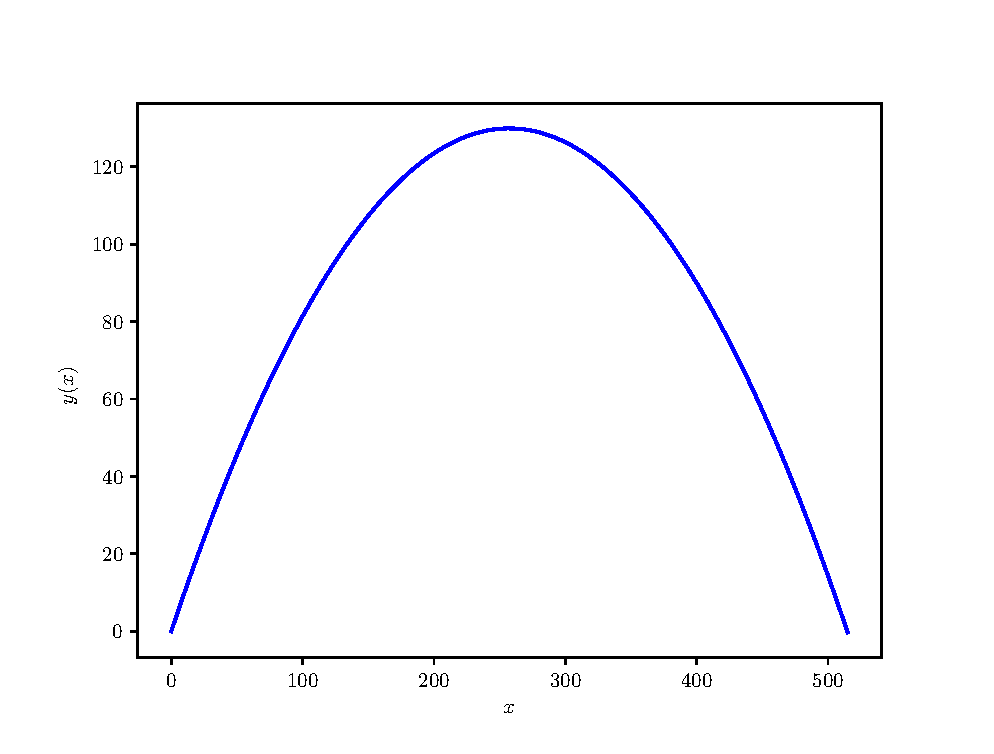
\includegraphics[width=\textwidth]{Figure_1.eps}
 \caption{Simulated trajectory $y(x)$ for the system without friction. The used integrator is the Euler scheme.}
 \label{fig:fig1}
\end{figure}



\subsection{Influence of friction and wind}
To account for friction, the function which calculates the force is modified in the following way:
\begin{lstlisting}
def force(mass, gravity, v, gamma, v_0):
   ret = np.array([0.0, -mass * gravity])
   ret -= gamma * (v - v_0)
   return ret
\end{lstlisting}
Because the force is now not constant anymore along the trajectory (it varies with the velocity $\mathbf{v}$), the function for the Euler step has to be modified as well:
\begin{lstlisting}
def step(x, v, dt, mass, gravity, gamma, v_0):
   x += v * dt
   f = force(mass, gravity, v, gamma, v_0)
   v += f / mass * dt
   return x, v
\end{lstlisting}
In contrast to the previous task, the force is now evaluated every time the Euler step is called.

\begin{figure}[H]
 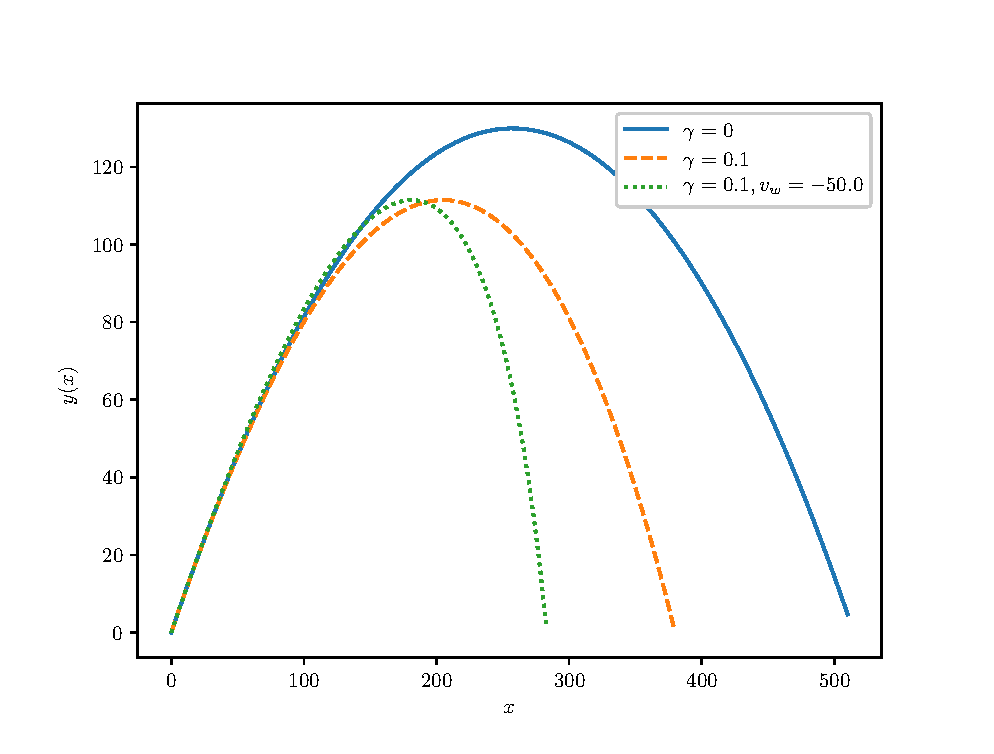
\includegraphics[width=\textwidth]{Figure_2.eps}
 \caption{Simulated trajectories $y(x)$ for a friction coefficient $\gamma=0.1$ and different values of the wind speed $v_w$. The used integrator is the Euler scheme.}
 \label{fig:fig2}
\end{figure}

\noindent\autoref{fig:fig2} shows simulated trajectories for the system without friction as well as for a system with friction coefficient $\gamma = 0.1$ and wind speeds of $v_w=0, -50.0$. Comparing the trajectory of the cannonball without friction to the ones with friction, we can easily see that the friction leads to both a decreased maximum height $y_\mathrm{max}$ and a decreased range $x_\mathrm{max}$. This is caused by the disspation of energy through the non-conservative friction force. We can also identify that the negative wind speed $v_w=-50.0$ leads to an even larger decrease of the range $x_\mathrm{max}$, this is also expected, because the friction force is proportional to the relative velocity of the air and the cannonball. Because the wind blows in the $x$-direction only, the maximum height $y_\mathrm{max}$ is the same for both cases.


\begin{figure}[t]
 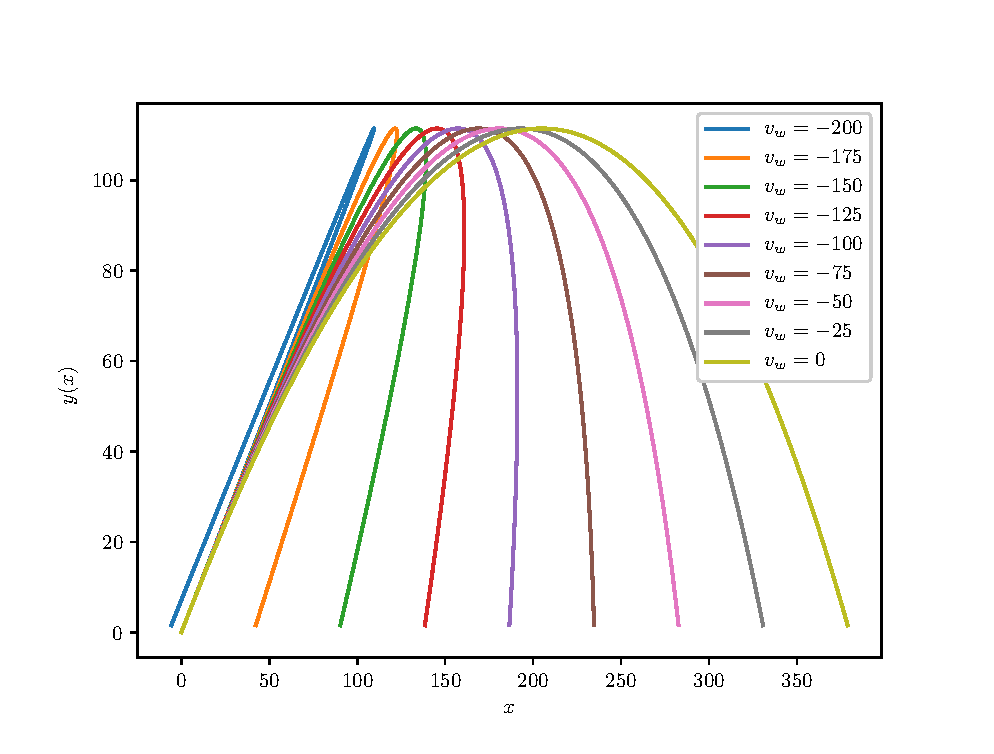
\includegraphics{Figure_3.eps}
 \caption{Simulated trajectories $y(x)$ for different values of the friction coefficient $\gamma$ and the wind speed $v_w$. For $v_w= -200$, the cannonball hits the ground closely to the starting point. The used integrator is the Euler scheme.}
 \label{fig:fig3}
\end{figure}

In \autoref{fig:fig3} we see multiple trajectories for $\gamma=0.1$ and different wind speeds. As the wind speed becomes more negative, the range of the cannonball becomes smaller because the friction increases. For $v_w\approx 200$ it hits the ground at its starting point.



\section{Solar system}
\subsection{Simulating the solar system with the Euler scheme}
The gravitational force between two particles is calculated using this function:
\begin{lstlisting}
def force(r_ij, m_i, m_j, g):
   return - g * m_i * m_j * r_ij / np.linalg.norm(r_ij) ** 3
\end{lstlisting}
To calculate all the forces on all the particles, the following function is used.
\begin{lstlisting}
def forces(x, masses, g):
   ret = np.zeros(x.shape)

   for i in range(len(x)):
       for j in range(i + 1, len(x)):
           f = force(x[j] - x[i], masses[i], masses[j], g)
           ret[i] -= f
           ret[j] += f

   return ret
\end{lstlisting}
The function returns an array which contains all forces.

A small modification of the Euler step is necessary because the particles have different masses:
\begin{lstlisting}
def step_euler(x, v, dt, mass, g):
    x += v * dt
    f = forces(x, mass, g)
    # calculate acceleration per coordinate dimension
    f[:, 0] /= mass
    f[:, 1] /= mass
    v += f * dt
    return x, v
\end{lstlisting}




\begin{figure}[t]
 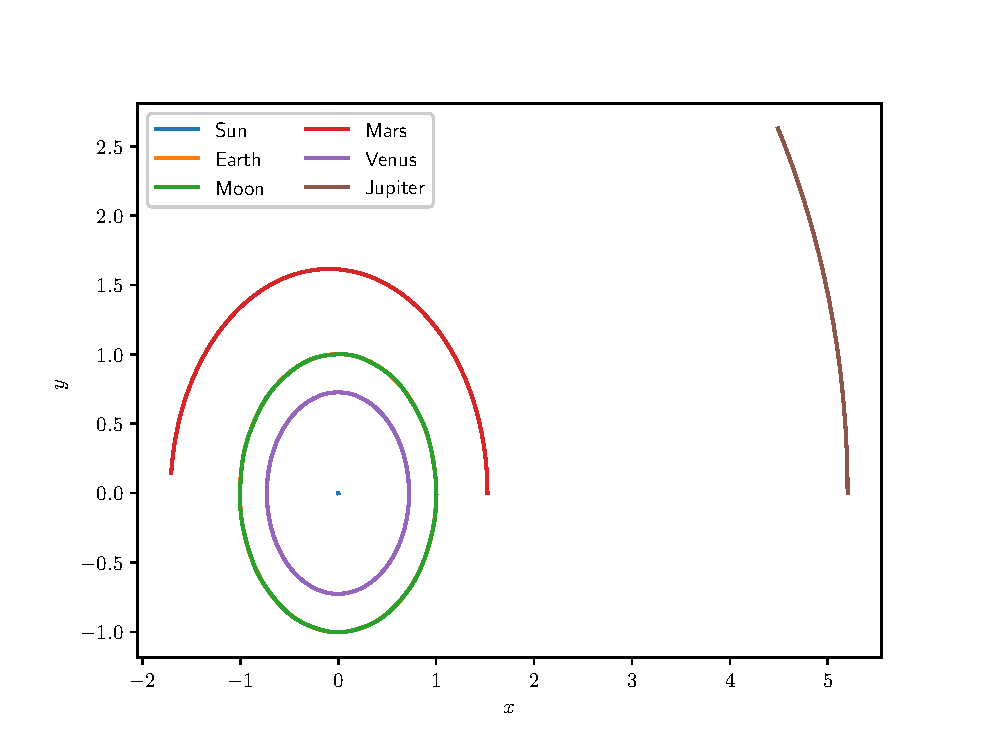
\includegraphics{Figure_4.eps}
 \caption{}
 \label{fig:fig4}
\end{figure}

\noindent In simulations with many particles, the computationally most expensive step is the evaluation of the forces $\mathbf{F}_{ij}$. For a system of $n$ particles, the complexity of this task scales like $\mathcal{O}\left(n^2\right)$ because the pairwise forces $\mathbf{F}_{ij}$ have to be evaluated for every of the $n(n-1)$ possible combination of $i,j$ (or at least half of them using Newton's third law).

\subsection{Integrators}
\subsubsection{Velocity Verlet algorithm}
The Velocity Verlet algorithm can be derived in the following way: For the positions $\mathbf{x}$, we perform a Taylor expansion up to the second order in $\Delta t$:
\begin{align}
\begin{split}
 \mathbf{x}(t + \Delta t) &= \mathbf{x}(t) + \dot{\mathbf{x}}(t)\cdot \Delta t + \frac{\ddot{\mathbf{x}}(t)}{2}\cdot \Delta t^2 + \mathcal{O}(\Delta t^3)\\
 &= \mathbf{x}(t) + \mathbf{v}(t)\cdot \Delta t + \frac{\mathbf{a}(t)}{2}\cdot \Delta t^2 + \mathcal{O}(\Delta t^3)
 \end{split}
 \label{eq:x}
\end{align}
For the velocites $\mathbf{v}$, we also perform a Taylor expansion up to the second order:
\begin{align}
\begin{split}
 \mathbf{v}(t + \Delta t) &= \mathbf{v}(t) + \dot{\mathbf{v}}(t)\cdot \Delta t + \frac{\ddot{\mathbf{v}}(t)}{2}\cdot \Delta t^2 + \mathcal{O}(\Delta t^3)\\
 &=\mathbf{v}(t) + \mathbf{a}(t)\cdot \Delta t + \frac{\ddot{\mathbf{v}}(t)}{2}\cdot \Delta t^2 + \mathcal{O}(\Delta t^3)
\end{split}
 \label{eq:v}
\end{align}
To get an expression for $\ddot{\mathbf{v}}(t)$, we perform a Taylor expansion of $\dot{\mathbf{v}}(t + \Delta t)$:
\begin{align}
 \dot{\mathbf{v}}(t + \Delta t) = \dot{\mathbf{v}}(t) + \ddot{\mathbf{v}}(t)\cdot \Delta t + \mathcal{O}(\Delta t^2)
\end{align}
We can solve this expression for $\ddot{\mathbf{v}}(t)$:
\begin{align}
 \ddot{\mathbf{v}}(t) = \frac{\dot{\mathbf{v}}(t+\Delta t) - \dot{\mathbf{v}}(t)}{\Delta t} + \mathcal{O}(\Delta t) = \frac{\mathbf{a}(t+\Delta t) - \mathbf{a}(t)}{\Delta t} + \mathcal{O}(\Delta t)
\end{align}
Plugging $\ddot{\mathbf{v}}(t)$ into \autoref{eq:v}, we get
\begin{align}
 \mathbf{v}(t + \Delta t) &=\mathbf{v}(t) + \mathbf{a}(t)\cdot \Delta t + \frac{\mathbf{a}(t+\Delta t) + \mathbf{a}(t)}{2} \cdot\Delta t^2 + \mathcal{O}(\Delta t^3)
 \label{eq:v2}
\end{align}
\autoref{eq:x} and \autoref{eq:v2} define the Velocity Verlet algorithm.
\subsubsection{Verlet algorithm}
The Verlet algorithm which was presented in the lecture can also be derived from the Velocity Verlet algorithm. Using \autoref{eq:x}, we can write $\mathbf{x}(t)$ as
\begin{align}
...
\end{align}


As we can see in ..., the Verlet algorithm needs the positions $\mathbf{x}(t)$ and $\mathbf{x}(t-\Delta t)$ to calculate the position $\mathbf{x}(t+\Delta t)$. However, the inital conditions only include the position at exactly one point in time $t_0$, this means that the initial conditions are not sufficient to solve the problem with the Verlet algorithm. To get the value of $\mathbf{x}(t_0-\Delta t)$ we have to use another integrator like the Euler scheme, this results in a bigger error.

\subsubsection{Implementation of the symplectic Euler algorithm}

\subsubsection{Implementation of the Velocity Verlet algorithm}


\subsection{Long-term stability}

\end{document}
